\chapter{Die Monte Carlo Methode}
\rhead{Die Monte Carlo Methode}
\begin{refsection}
\chapterauthor{Dorian Amiet, Hannes Badertscher}
\lstdefinestyle{C}{
  belowcaptionskip=1\baselineskip,
  breaklines=true,
  frame=L,
  xleftmargin=\parindent,
  language=C,
  showstringspaces=false,
  basicstyle=\footnotesize\ttfamily,
  keywordstyle=\bfseries\color{green!40!black},
  commentstyle=\itshape\color{purple!40!black},
  identifierstyle=\color{blue},
  stringstyle=\color{orange},
  numberstyle=\ttfamily\tiny
}

\section{Einleitung}
Der Monte Carlo Algorithmus ist ein Verfahren zur L"osung numerischer
Probleme durch das Ziehen von Zufallszahlen. Die Idee, mathematische
bzw. physikalische Probleme mit einem stochastischen Sampling-Verfahren
zu approximieren, stammt vom polnisch-amerikanischen Mathematiker
Stanisław Marcin Ulam (1909 -- 1984), welcher zu dieser Zeit im Los
Alamos National Labaratory arbeitete. Seine Idee und wie es dazu kam,
beschrieb er folgendermassen:

\begin{quote}
``The first thoughts and attempts I made to practice [the
Monte Carlo method] were suggested by a question which occurred to me in
1946 as I was convalescing from an illness and playing solitaires. The
question was what are the chances that a Canfield solitaire laid out with
52 cards will come out successfully? After spending a lot of time trying
to estimate them by pure combinatorial calculations, I wondered whether
a more practical method than “abstract thinking” might not be to lay
it out say one hundred times and simply observe and count the number of
successful plays. This was already possible to envisage with the beginning
of the new era of fast computers, and I immediately thought of problems
of neutron diffusion and other questions of mathematical physics, and
more generally how to change processes described by certain differential
equations into an equivalent form interpretable as a succession of random
operations. Later... [in 1946, I ] described the idea to John von Neumann
and we began to plan actual calculations.'' - Stan Ulam, 1983
\end{quote}

Monte Carlo Methoden kommen "uberall zum Einsatz, wo deterministische
Algorithmen entweder zu komplex sind oder gar nicht existieren. Dank
zunehmender Rechenleistung sind in den letzten Jahren Simulationen wie
globale Klimamodelle m"oglich geworden. Typische Anwendungen des Monte
Carlo Algorithmus umfassen u.a.

\begin{itemize}
\item Numerische Integration
\item Simulation von dynamischen Prozessen
\item Simulation von Gleichgewichtszust"anden (z.B. mit Metropolis-Algorithmus)
\item Statistische Untersuchung von Zufallsverteilungen
\end{itemize}

\section{Funktionsprinzip}
Die Monte Carlo Methode ist ein Überbegriff f"ur verschiedene Algorithmen
zur numerischen Berechnung / Simulation mittels Zufallsereignissen. Ein
weit verbreiteter und sehr flexibler Ansatz ist das sogenannte Hit-or-Miss
Verfahren. Dabei werden Zufallszahlen generiert und gepr"uft, ob diese
eine bestimmte Bedingung erf"ullen oder nicht. Mit dem Verh"altnis Hit /
Miss wird das gew"unschte Ergebnis approximiert.

\subsection{Numerische Integration} \label{subsec:numIntegration}
Einer der wichtigsten Anwendungsbereiche der Monte Carlo Methode ist
die numerische Berechnung von Integralen. Dazu werden innerhalb des
Definitionsbereich der zu integrierenden Funktion Zufallsereignisse
generiert. Generell kann ausgesagt werden, dass das Integral

\begin{equation}
	I = \int_a^b f(x) dx
\end{equation} 

mit $N$ im Intervall $[a,b]$ gleichverteilten Zufallszahlen $x_i$ durch

\begin{equation}
	\hat{I} = (b-a) \cdot \frac{1}{N} \sum_{i=1}^{N} f(x_i)
\end{equation}

approximiert werden kann. Der relative Fehler sinkt dabei mit $1 /
\sqrt{N}$. W"ahrend f"ur analytisch l"osbare Integrale und solche mit
kleinen Dimensionen ($\leq 4$) andere M"oglichkeiten oft schneller sind,
ist die Monte Carlo Methode besonders bei hohen Dimensionen oder sehr
komplizierten Integrationsgrenzen verbreitet.

Der Algorithmus l"asst sich sehr einfach beschreiben:

\begin{enumerate}
\item Finde das Maximum $f_{\max}$ der Funktion $f(x)$.
\item Erzeuge $N$ im Intervall $[a,b]$ gleichverteilte Zufallszahlen $x_i$.
\item Erzeuge f"ur jedes $x_i$ ein in $[0,f_{\max}]$ gleichverteiltes $y_i$.
\item Falls $y_i < f(x_i)$ wird das $x_i$ akzeptiert, sonst verworfen.
\item Wenn $N^*$ die Anzahl der akzeptierten $x_i$ ist, dann ist $F =
\frac{N^*}{N}(b-a)f_{\max}$.
\end{enumerate}

Abbildung \ref{fig:integration_histogram} zeigt eine beliebige Funktion
(rot), sowie die akzeptierten Ereignisse (blau) und die nicht akzeptierten
Ereignisse (gr"un).

\begin{figure}[htbp]
	\centering
	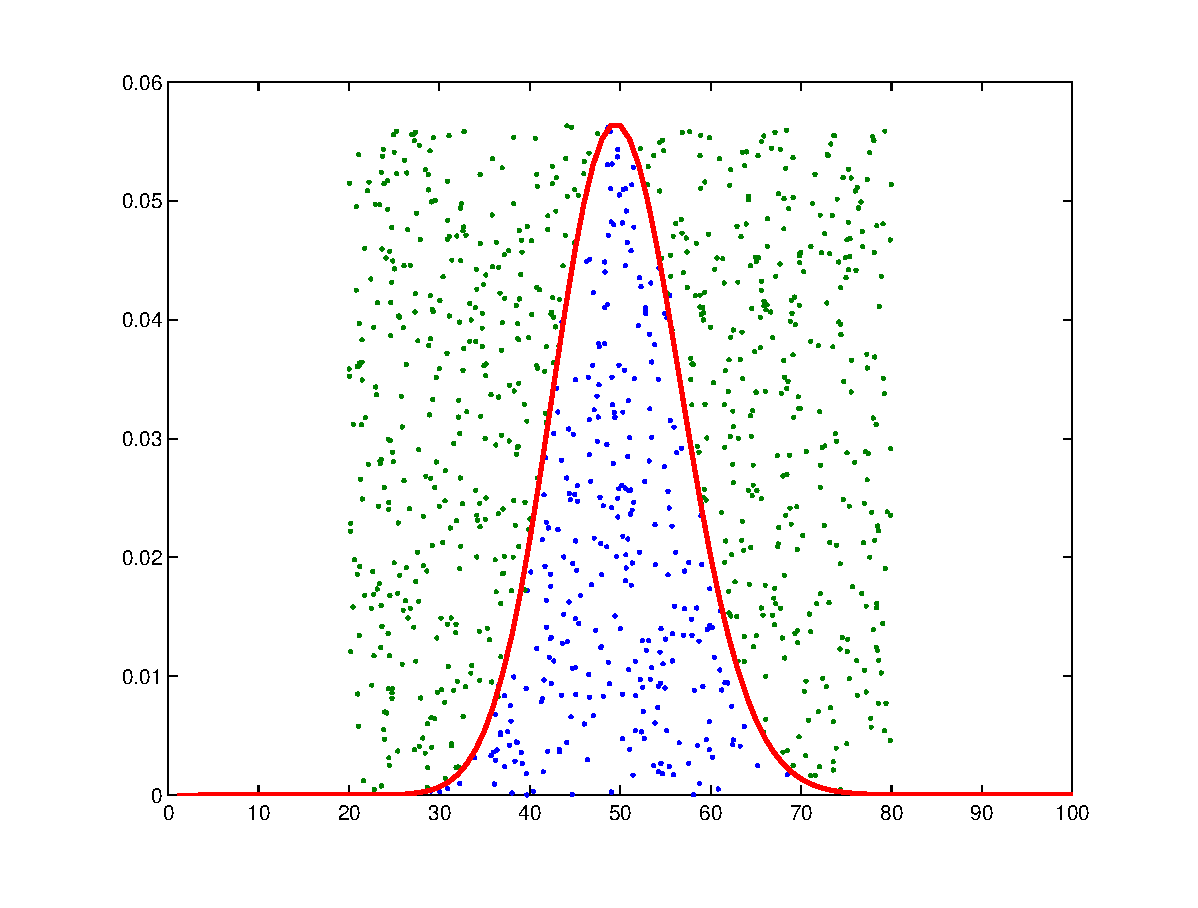
\includegraphics[width=7cm]{montecarlo/images/integration_poisson.eps}
	\caption{Monte Carlo Integration einer Funktion}
	\label{fig:integration_histogram}
\end{figure}

\subsection{Absch"atzung des Wertes von Pi}
Als Einf"uhrungsbeispiel f"ur die Monte Carlo Methode wird die Zahl $\pi$
mit einer Hit-or-Miss Methode abgesch"atzt. Ein Kreis mit Radius $r$
hat eine Grundfl"ache von $A_{\text{Kreis}} = \pi r^{2}$.  Damit muss
in einem Intervall von $[-r,+r]$ integriert werden, was eine Fl"ache
von $A_{\text{Quadrat}} = 4r^2$ ergibt. Damit l"asst sich $\pi$
approximieren als

\begin{equation}
	\hat{\pi} = \frac{A_{\text{Kreis}}}{r^2} = 4 \frac{A_{\text{Kreis}}}{A_{\text{Quadrat}}}
\end{equation}

Das Verh"altnis der Fl"ache des Kreises zur Fl"ache des Quadrats
entspricht der Wahrscheinlichkeit, dass ein Paar von Zufallszahlen
$(x_i,y_i)$ mit $x_i,y_i \leq r$ innerhalb des Kreises mit Radius $r$
liegen. Dies wird mit folgender Formel "uberpr"uft:

\begin{equation}
	x^2 + y^2 \leq r^2
	\label{equ:innerhalbKreis}
\end{equation}

\begin{figure}[htbp]
	\centering
	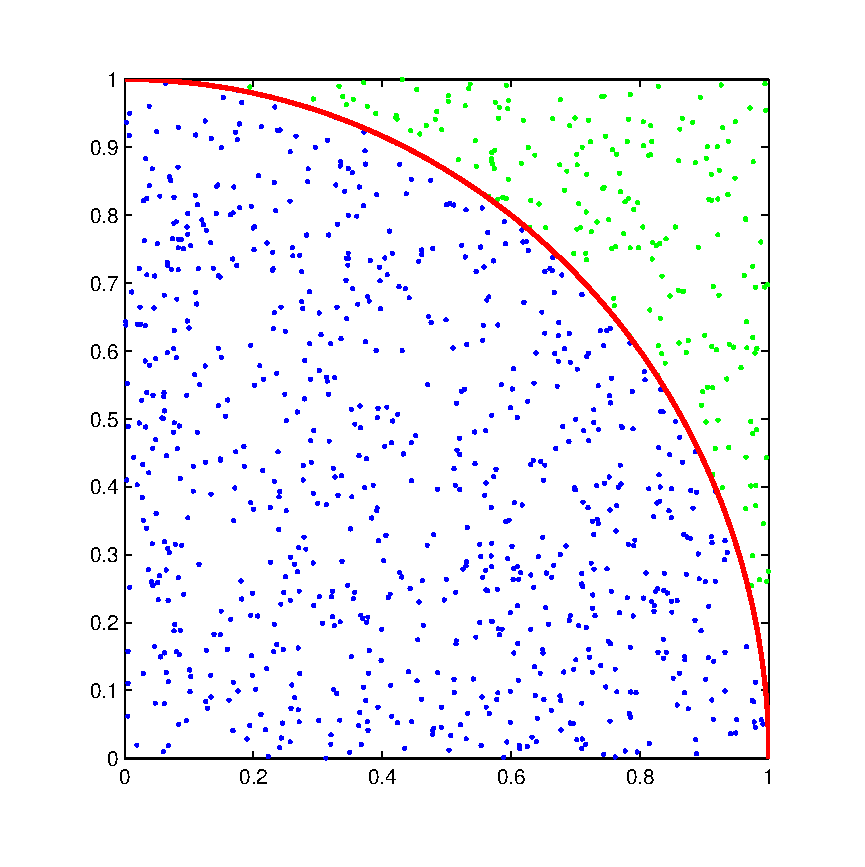
\includegraphics[width=6cm]{montecarlo/images/kreis_hitmiss.eps}
	\caption{Kreis}
	\label{fig:KreisHitMiss}
\end{figure}

Dank der Symmetrie des Kreises kann das Problem offensichtlich auf den
ersten Quadranten reduziert werden. F"ur $N$ Iterationen, von welchen
$k$ die Bedingung \ref{equ:innerhalbKreis} erf"ullen, ergibt sich somit
folgende Absch"atzung f"ur $\pi$:

\begin{equation}
	\hat{\pi} = 4 \cdot \frac{k}{N}
\end{equation}


\subsubsection{Weitere Anwendungen}
Besonders in der Teilchenphysik - aus welcher die Monte Carlo Methode
bekannterweise stammt - wird die Monte Carlo Methode sehr h"aufig
angewandt. Dort stellt sich das Problem, dass verschiedene Prozesse
zwischen einzelnen Teilchen auftreten k"onnen. Diese Prozesse oder
Ereignisse werden als Inputs $I_i$ bezeichnet. Ein Detektor misst nun
gewisse Outputs $O_j$. Dabei interagieren die Inputs $I_i$ jedoch auch
mit dem Detektor. Da in der Quantenmechanik nicht alles deterministisch
abl"auft, m"ussen probabilistische Aussagen gemacht werden, d.h. $P(O_j
| I_i)$ gesch"atzt werden. Auch wenn verschiedene Zwischenschritte das
Resultat $O_j$ beeinflussen, kann aufgrund der Wahrscheinlichkeit $P(O_j |
I_i)$ und der Wahrscheinlichkeit des Outputs $P(O_j)$ eine Aussage "uber
den Input $I_i$ gemacht werden. Solche Methoden werden u.a. verwendet,
um das Higgs Boson nachzuweisen. 

In der Versicherungsbranche ist die Monte Carlo Methode ebenso
verbreitet. Dabei stellt sich ein "ahnliches Problem: Ein Schadensszenario
($I_i$), z.B. ein Hochwasser, f"uhrt zu direkten Sch"aden und "uber
komplizierte Zusammenh"ange zu Folgesch"aden. Ein direkter Zusammenhang
zwischen einem Input $I_i$ und einem finanziellen Schaden $O_j$ ist
schwierig zu berechnen. Mit einer Monte Carlo Simulation kann die
Wahrscheinlichkeit eines Schadens $P(O_j | I_i)$ simuliert werden und
daraus eine Versicherungspr"amie berechnet werden.



\section{Implementation}
\subsection{Implementation in C}
Die Implementation dieses Beispiels in C ist relativ kurz und
"ubersichtlich: Über $N$ Iterationen wird jeweils ein Paar von
Zufallszahlen $(x,y)$ generiert und die Gleichung
\ref{equ:innerhalbKreis}: $x^2 + y^2$ berechnet. Ist das Resultat $\leq1$,
wird eine Summe erh"oht. Das Resultat ist schlussendlich die Summe geteilt
durch die Anzahl Iterationen $N$ mal 4. Da diese L"osung nicht parallel
abl"auft, steigt der Rechenaufwand linear mit der Anzahl Iterationen.

Die Effizienz $\varepsilon$ des Hit-or-Miss Algorithmus l"asst sich
mit der Anzahl Hits $k$ und der Iterationen $N$ gem"ass Gleichung
\ref{equ:effizienz_hitnmiss} beschreiben.
\begin{equation}
	\varepsilon = \frac{k}{N}
	\label{equ:effizienz_hitnmiss}
\end{equation} 
Eine Effizienz von $\varepsilon=1$ w"urde bedeuten, dass das
Definitionsgebiet der Zufallszahlen $\Omega$ genau der Zielfunktion
entspricht. Wird $\Omega$ sehr gross gew"ahlt, ist die Wahrscheinlichkeit
eines Hits sehr gering und es sind viele Iterationen notwendig, um das
korrekte Resultat zu erreichen. Der relative Fehler der Sch"atzung wird
gem"ass Gleichung \ref{equ:relativer_Fehler} berechnet.

\begin{equation}
	\text{Relativer Fehler} = \sqrt{\frac{1-\varepsilon}{k}} 
	\label{equ:relativer_Fehler}
\end{equation}

F"ur hohe $N$ wird der Fehler mit einem Faktoren $1 / \sqrt{N}$ gegen $0$
konvergieren. Dies ist in Abbildung \ref{fig:Fehler} klar ersichtlich.

\begin{figure}[ht!]
    \centering
    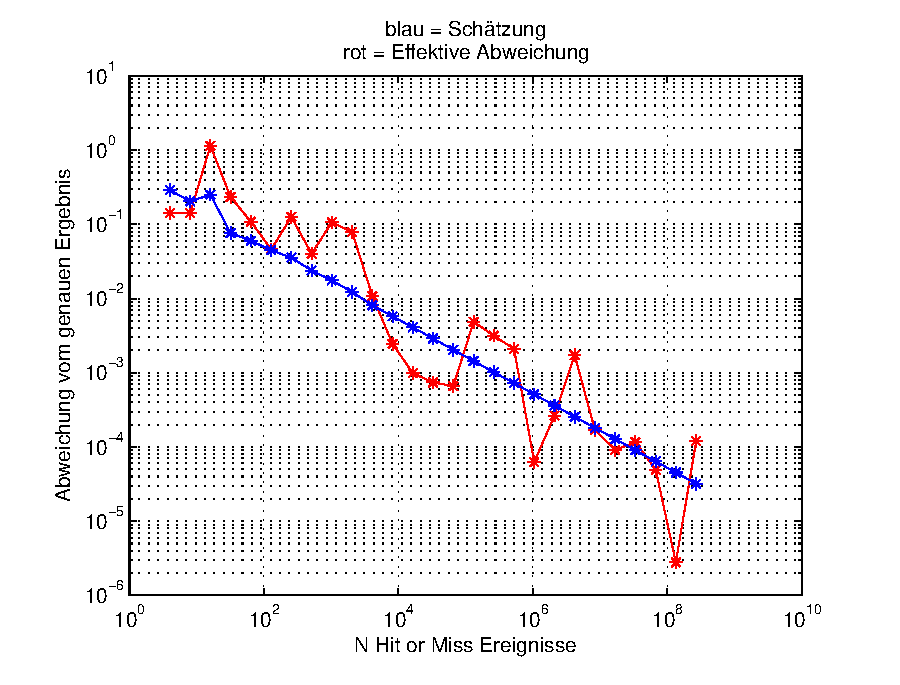
\includegraphics[width=8cm]{montecarlo/images/Fehler.eps}
    \caption{Betrag der Abweichung}
    \label{fig:Fehler}
\end{figure}
\newpage

\subsection{Genauigkeit des Sch"atzers}

Um die Genauigkeit der Fehlerabweichung besser absch"atzen zu k"onnen,
wird die Simulation 1000 mal durchgef"uhrt und die gemittelte effektive
Abweichung mit der Sch"atzung verglichen.

\begin{figure}[ht!]
    \centering
    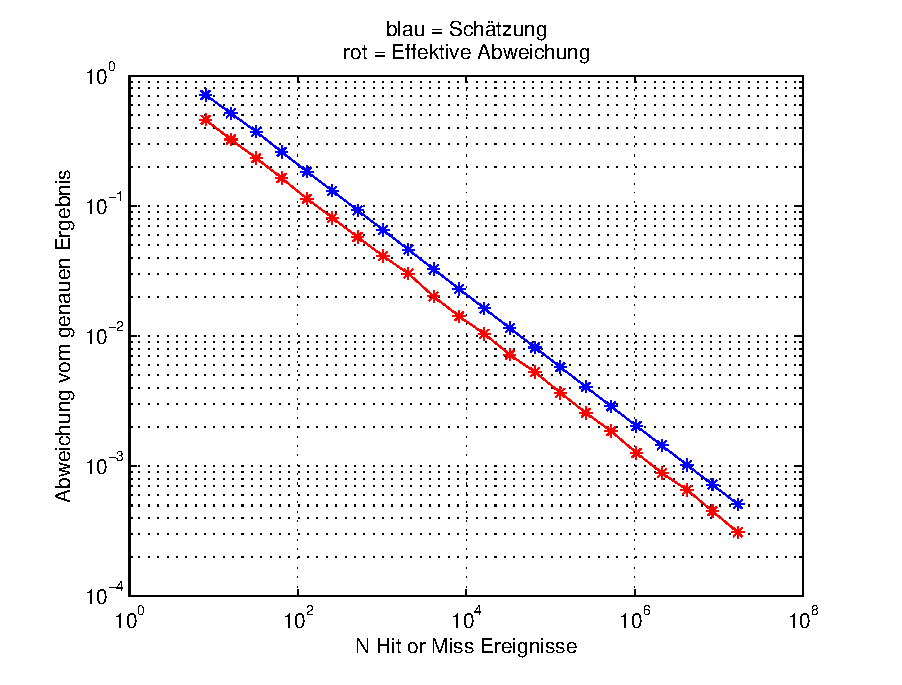
\includegraphics[width=8cm]{montecarlo/images/Fehler_gemittelt.eps}
    \caption{Betrag der Abweichung, gemittelt}
    \label{fig:Fehler_gemittelt}
\end{figure}

Dabei zeigt sich, dass die Sch"atzung ca. um den Faktor 2 h"oher liegt als
die Abweichungen der Simulationsergebnisse. Zumindest die Gr"ossenordnung
des Sch"atzers stimmt somit. Um zu illustrieren, wie der Faktor zustande
kommen k"onnte, wird ein Histogramm der Fehlerabweichung gemacht. Dazu
werden eine Million Simulationen mit N=1000 durchgef"uhrt und in die
Betr"age der Abweichung in ein Histogramm eingetragen. In Abbildung
\ref{fig:Histogramm} ist ersichtlich, dass die Streuung ziemlich
hoch ist. Es tauchen Werte auf, welche das zehnfache des Sch"atzers
betragen. Somit ist der Sch"atzer sowieso nur als Gr"ossenordnung zu
verstehen, da ein einzelnes Simulationsergebnis wesentlich ungenauer
sein kann.

\begin{figure}[ht!]
    \centering
    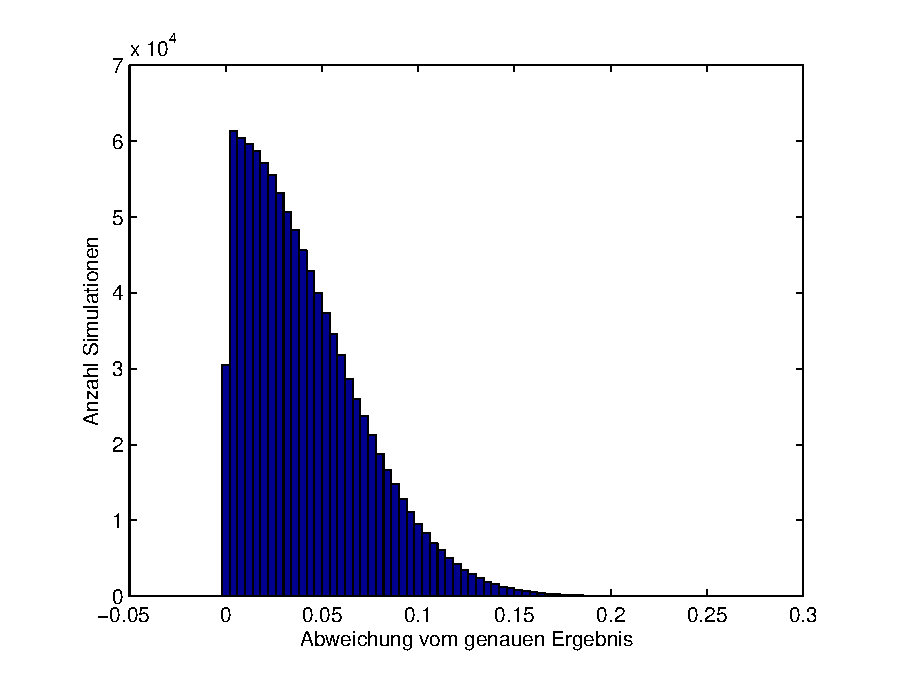
\includegraphics[width=8cm]{montecarlo/images/Histogramm.eps}
    \caption{Betr"age des Effektiven Fehlers bei N = 1000, Fehlersch"atzung = 0.0414}
    \label{fig:Histogramm}
\end{figure}


\subsection{Implementation in OpenCL}
Bei der Monte Carlo Analyse werden sehr viele komplett unabh"angige
Berechnungen durchgef"uhrt. Dadurch ist OpenCL perfekt geeignet, um das
Problem zu parallelisieren. Die gr"osste Schwierigkeit dabei ist die
Generierung von Zufallszahlen auf der GPU.

\subsubsection{Ansatz I: Zufallszahlen auf CPU}
Die einfachste L"osung f"ur das Problem ist es, auf der CPU qualitativ
hochwertige Zufallszahlen zu generieren und in einem Array an OpenCL
zu "ubergeben. Jeder Worker liest seine zwei Zufallszahlen aus und
rechnet das Resultat f"ur diesen Punkt aus. So ist sichergestellt,
dass die Zufallszahlen wirklich zuf"allig sind und das Resultat
gegen den korrekten Wert konvergiert. Die Nachteile sind, dass die
Berechnung der Zufallszahlen seriell und somit langsam ist, sowie der
hohe Speicherverbrauch. Dieser kann um einen Faktor 2 reduziert werden,
indem nur eine Zufallszahl "ubergeben wird und jeder Worker sich eine
zweite Zahl berechnet.

Wird diese Variante mit C bzw. OpenCL umgesetzt, stellen sich die
erwarteten Resultate ein: Die Rechenzeit steigt linear mit der Anzahl
Punkte, die Berechnung ist jedoch deutlich schneller als bei serieller
Berechnung auf der CPU. Mit 48.909 Mio Berechnungen pro Sekunde ist
die parallelisierte Version um Faktor 5 schneller  als die serielle
Implementation.

\begin{figure}[ht!]
	\centering
	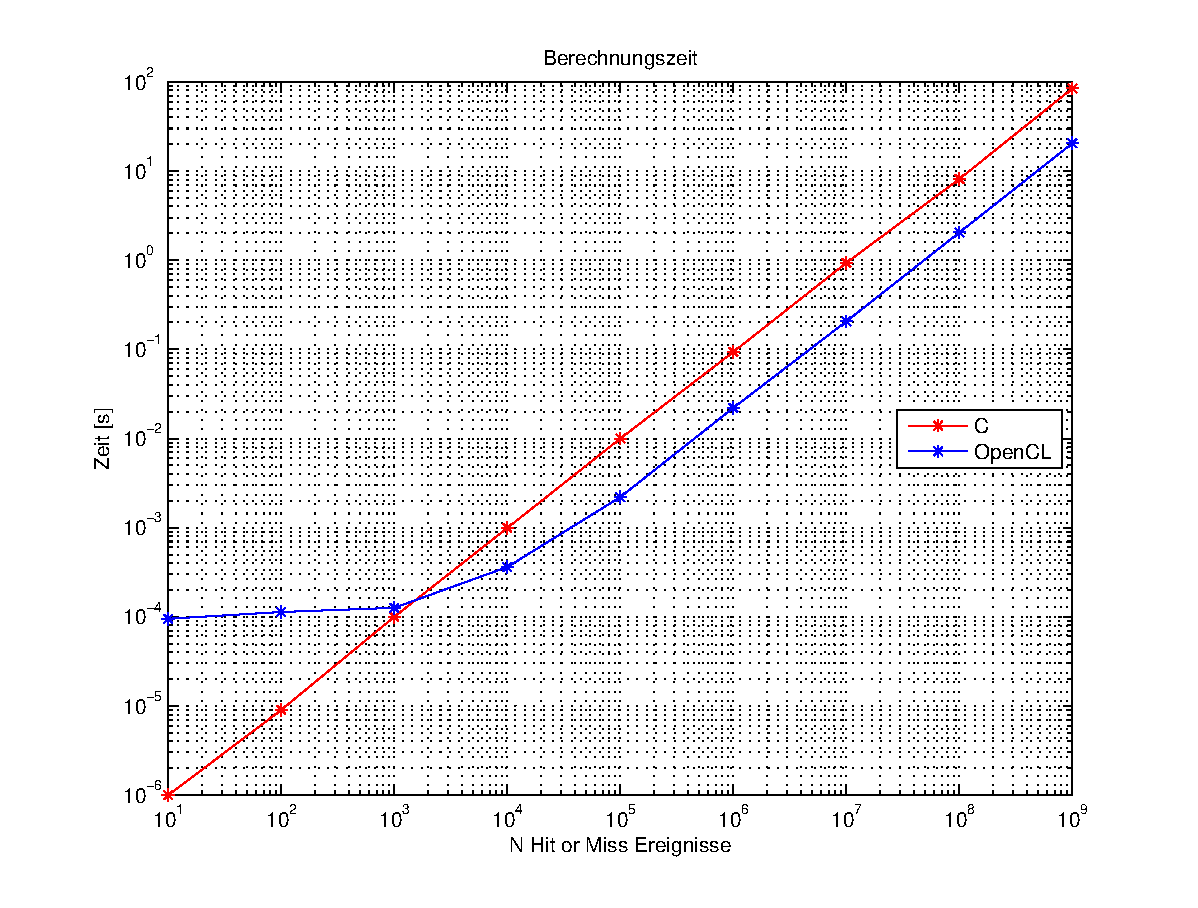
\includegraphics[width=8cm]{montecarlo/images/Berechnungszeit_OpenCL.eps}
	\caption{Berechnungszeit mit OpenCL}
	\label{fig:OpenCL_Berechnungszeit}
\end{figure}


\subsubsection{Ansatz II: Zufallszahlen auf GPU}
Da Zufallszahlen mathematisch berechnet werden, liegt es nahe,
diese auf der GPU zu berechnen. Als Startwert (seed), kann z.B. die
Worker-ID verwendet werden. So verf"ugen alle Worker "uber unabh"angige
Zufallszahlen. Die meisten Algorithmen sind jedoch nur dazu geeignet,
von einem Startwert aus eine lange Folge unabh"angiger Zufallszahlen zu
berechnen. Wird der Algorithmus nach nur 2 Werten mit einem anderen
Startwert neu gestartet, ergibt sich kein besonders zuf"alliges
Muster. Abbildung \ref{fig:OpenCL_ID_Seed} zeigt den Ausgang eines
Zufallszahlengenerators in Abh"angigkeit des Startwertes. Werden diese
Werte f"ur die Monte Carlo Simulation verwendet, wird das Ergebnis nicht
gegen den korrekten Wert konvergieren.

\begin{figure}[ht!]
	\centering
	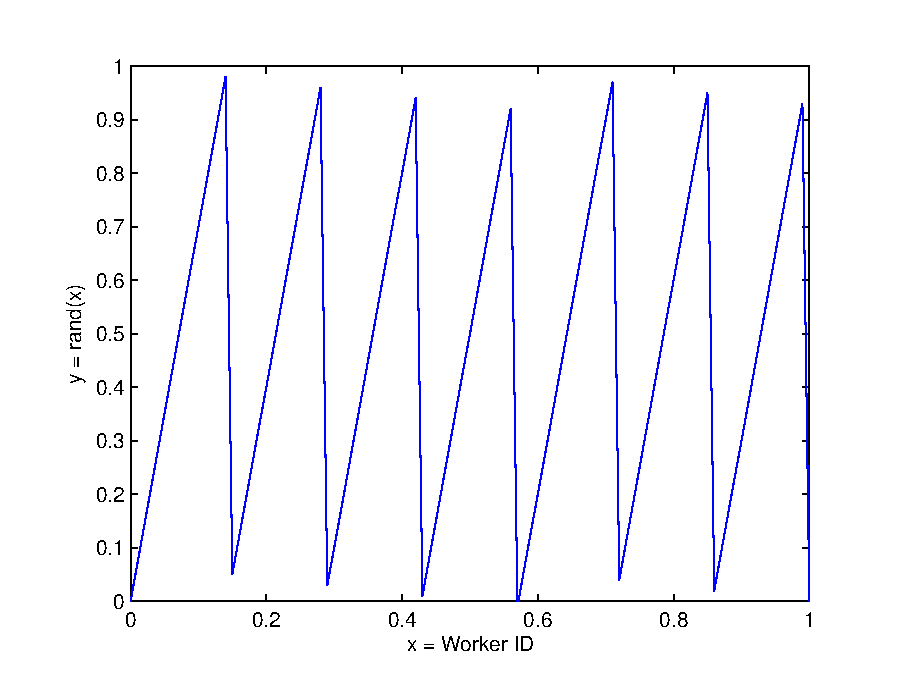
\includegraphics[width=8cm]{montecarlo/images/idAsSeed.eps}
	\caption{Zufallszahlen auf GPU mit Worker-ID als Seed}
	\label{fig:OpenCL_ID_Seed}
\end{figure}

\subsubsection{Ansatz III: Mischform}
Die beste L"osung liegt in einer Mischform der beiden Ans"atze: Auf
der CPU wird eine geringe Anzahl qualitativ hochwertiger Zufallszahlen
generiert. Mit diesen k"onnen Zufallszahlen-Generatoren auf der GPU
initialisiert werden. Damit sich dieser Aufwand lohnt, wird pro Worker
nicht nur ein Punkt berechnet, sondern eine Serie von Punkten. Das
empfohlene Vorgehen lautet wie folgt:
\newpage
\begin{enumerate}
\item Absch"atzen der Anzahl n"otiger Iterationen $N$.
\item Bestimmen des Zielsystems und der Anzahl parallel ausf"uhrbarer
Workers $M$.
\item Generieren von $M$ hochwertiger Zufallszahlen auf der CPU.
\item Übergabe dieser $M$ Zahlen an OpenCL, Start des Kernels.
\item Jeder Worker berechnet $N/M$ Punkte und gibt das Resultat zur"uck.
\item Zusammenf"uhren und Auswerten der Resultate der einzelnen Worker
auf der CPU.
\end{enumerate}

Mit diesem Verfahren l"asst sich die vorhandene Hardware gut ausnutzen,
ohne Genauigkeit durch schlechte Zufallszahlen zu verlieren.

\section{Zufallszahlengeneratoren} 

\begin{quote}
``Anyone who considers arithmetical methods of producing random digits
is, of course, in a state of sin.'' - John von Neumann, 1951
\end{quote}

Die Generierung von Zufallszahlen ist absolut essentiell f"ur die Monte
Carlo Methode. In der analogen Welt bestehen verschiedene hervorragende
Zufallsgeneratoren, u.a. das thermische Widerstandsrauschen oder
radioaktive Zerfallsvorg"ange. So gab es in der Vergangenheit Ans"atze,
in welchen die Strahlung einer radioaktiven Quelle gemessen wurde und
daraus eine Folge von Zufallszahlen generiert wurde. Heute werden eher
Rauschgeneratoren mit Widerst"anden oder Dioden verwendet. In digitalen
Schaltungen wird teilweise der Ausgang eines metastabilen Flip-Flop als
Zufallszahlengenerator verwendet.

In Software ist es deutlich schwieriger, ``gute'' Random Number
Generators (RNGs) zu realisieren. Technisch gesehen sind Software
RNGs immer \textit{Pseudo} Random Number Generators (pRNGs),  denn
der Ausgangswert eines deterministischen Programms kann per Definition
nicht zuf"allig sein. Die Schwierigkeit ist es, Zahlen zu generieren,
die aus der Perspektive des Anwenders komplett zuf"allig sind, obwohl
sie eindeutig mathematisch definiert sind.

\subsection{Beurteilung von Zufallszahlen}
Die Qualit"at von Zufallszahlen kann nicht generell gemessen werden:
F"ur kryptographische Anwendungen sind ganz andere Qualit"atsmerkmale
n"otig als bei einer Monte Carlo Simulation. Es ist logisch, dass ein
Zufallszahlengenerator eine bestimmte Verteilungsfunktion, in der Regel
eine Gleichverteilung, erf"ullen muss. F"ur die Monte Carlo Methode sind
folgende Punkte wichtig:

Die Periodendauer, d.h. die Anzahl Zahlen bis sich eine Sequenz wiederholt
soll m"oglichst gross sein. Wenn $N$ Iterationen durchgef"uhrt werden,
m"ussen mindestens $N$ unabh"angige Zufallsvektoren generiert werden
k"onnen.

Gewisse Zufallszahlengeneratoren sind in einer Dimension zwar qualitativ
gut, in mehreren jedoch nicht. Wenn also zwei aufeinanderfolgende
Zufallszahlen als x,y-Koordinaten eines Punktes interpretiert werden,
sind diese Punkte nicht mehr gleichverteilt. F"ur die Monte Carlo Methode
ist es wichtig, dass die Eingangspunkte unabh"angig und gleichverteilt
sind. Eine graphische Darstellung eines ''guten`` Zufallszahlengenerators
in 2D ist in Abbildung \ref{fig:Zufallszahlen_gut} dargestellt.

\begin{figure}[htbp]
	\centering
	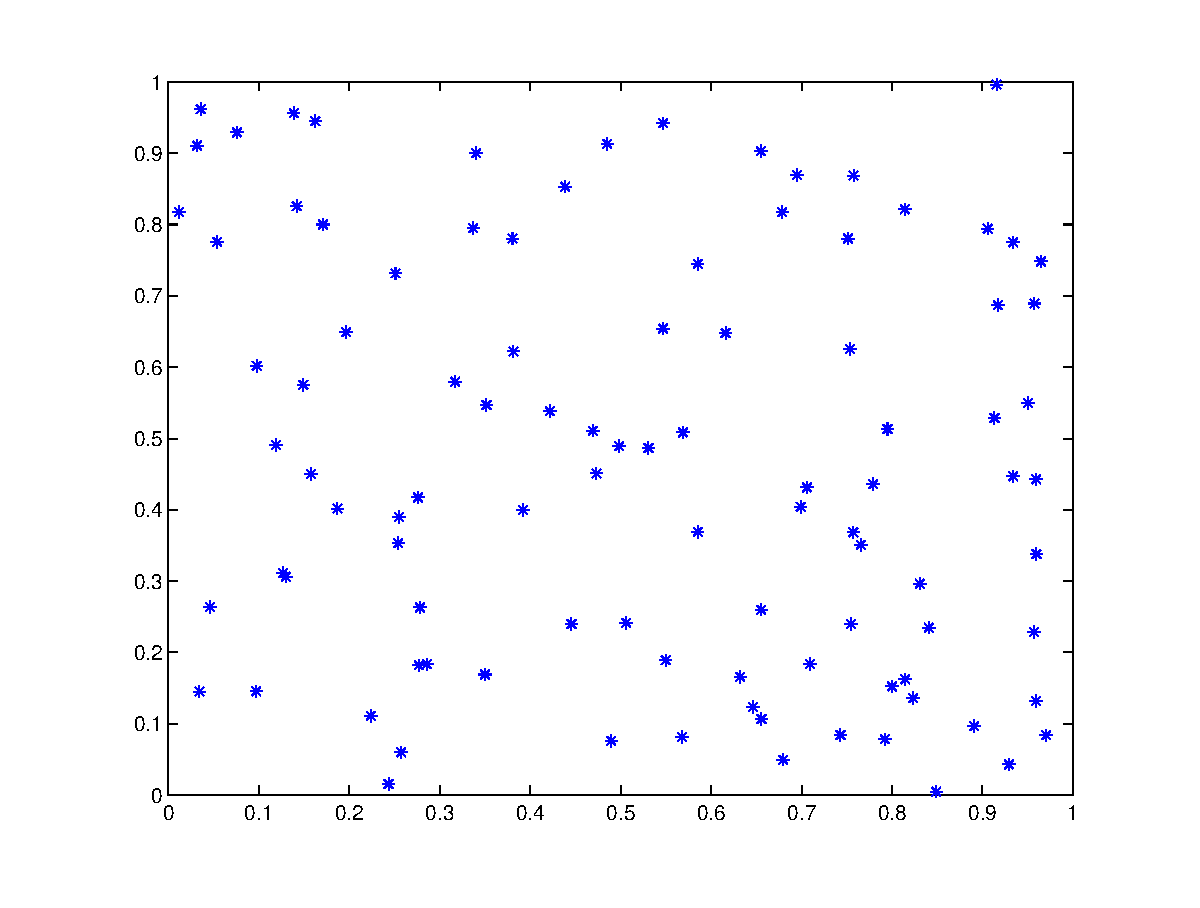
\includegraphics[width=8cm]{montecarlo/images/Zufallszahlen_gut.eps}
	\caption{Beispiel f"ur eine gute Verteilung aufeinanderfolgender Punkte}
	\label{fig:Zufallszahlen_gut}
\end{figure}

\subsection{Random-Device} \label{subsec:RandomDev}

Auf Unix-Systemen steht mit dem sog. Random-Device (\texttt{/dev/random})
ein Zufallszahlengenerator sehr hoher G"ute zur Verf"ugung. Dieser
sammelt das Rauschen von Ger"atetreibern in einem Entropie-Pool und
generiert daraus Zufallszahlen, welche auch h"ochsten Anforderungen im
Bereich der Kryptografie gen"ugen. Der Nachteil ist, dass sobald dieser
Entropie-Pool ersch"opft ist keine Zufallszahlen mehr generiert werden
k"onnen. Mit dem Device \texttt{/dev/urandom} wurde Abhilfe geschaffen,
was jedoch mit dem Nachteil erkauft wird, dass beim Unterschreiten einer
gewissen Entropie-Schwelle nur Pseudozufallszahlen generiert werden,
welche unter Umst"anden von einem potentiellen Angreifer berechnet werden
k"onnten. Den meisten Anforderungen gen"ugt dies jedoch trotzdem.

Das Random-Device kann von einem Programm wie ein File eingebunden
werden und Zufallszahlen daraus gelesen werden. F"ur viele Anwendungen
ist dies klar zu langsam, weshalb h"aufig das Random-Device nur als Seed
f"ur einen Pseudo-Random-Number-Generator verwendet wird.

Ein Code-Snippet zur Verwendung des Random-Device ist im Github-Repository
\cite{rng:githubRepo} zu finden.


\subsection{Multiplikativ kongruentielle Generatoren (LCG)} \label{subsec:LCG}
Eine der popul"arsten Methoden zur Generierung von Zufallszahlen ist die
multiplikativ kongruentielle Methode. Solche Generatoren werden h"aufig
als \textit{linear congruential generator (LCG)} bezeichnet. Dabei werden
Zufallszahlen rekursiv nach folgender Vorschrift berechnet:

\begin{equation}
	x_{i+1} = \left( a x_{i} + b \right) \mod{m}
	\label{equ:lcg_equation}
\end{equation}

Der Generator ist durch den Startwert $x_1$, den Faktor $a$,
das Inkrement $b$ und das Modul $m$ vollst"andig bestimmt. Ein LCG
generiert Zufallszahlen zwischen $0$ und $m-1$. F"ur viele Zwecke sind
gleichverteilte Zufallszahlen zwischen $0$ und $1$ gefragt. Diese werden
wie folgt berechnet:

\begin{align}
	y_i &= \frac{x_i}{m} \: &\text{for approx. uniformly distributed numbers  in } [0,1)\\
	y_i &= \frac{x_i}{m-1} \: &\text{for approx. uniformly distributed numbers in [0,1]}
\end{align} 

LCG Generatoren sind sehr stark von der Wahl der Konstanten $a$,$b$,$m$
abh"angig. Eine suboptimale Wahl kann zu einer sehr geringen Periode
und einer eindeutigen Korrelation aufeinanderfolgender Zahlen
f"uhren. Abbildung \ref{fig:lcg_verteilung} verdeutlicht dies anhand
eines LCG mit $a=11$, $b=0$ und $m=64$.

\begin{figure}[h]
	\centering
	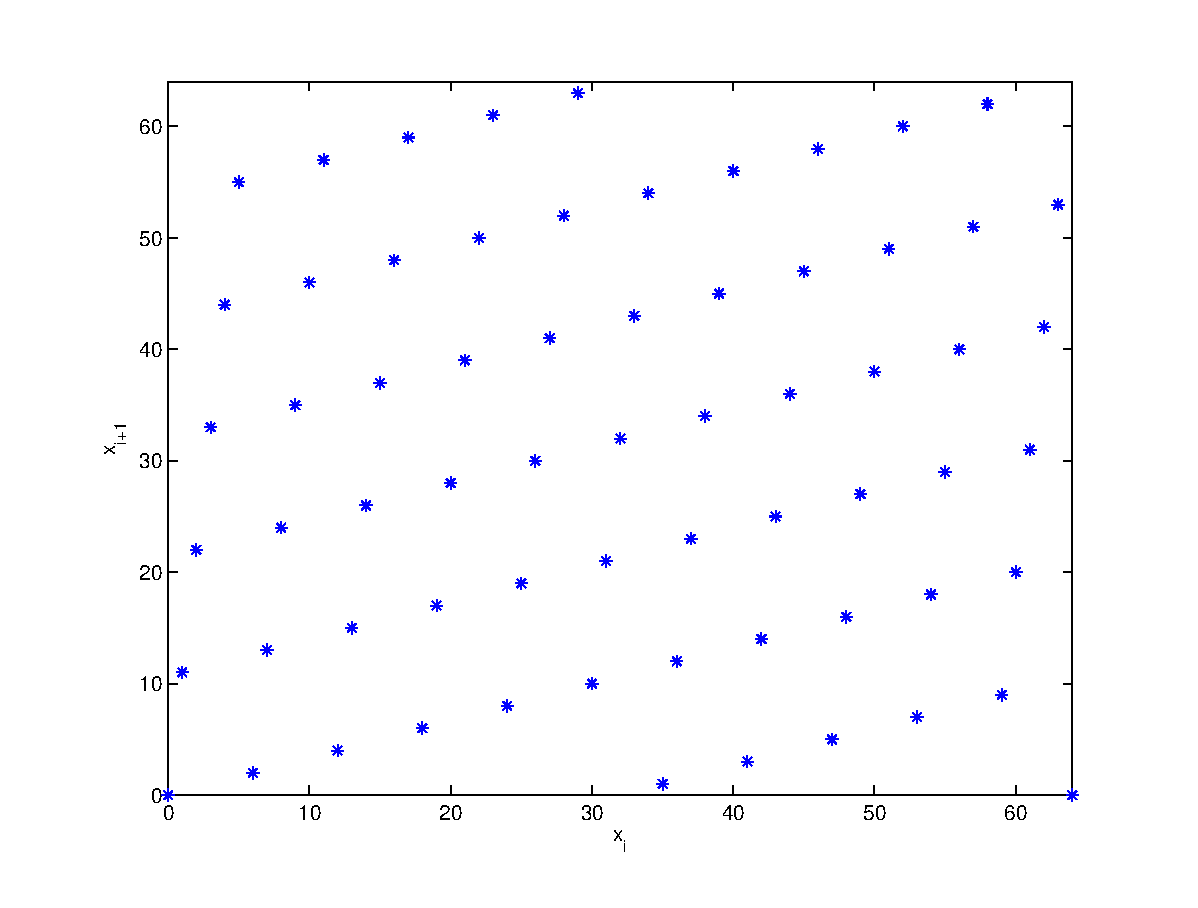
\includegraphics[width=8cm]{montecarlo/images/lcg.eps}
	\caption{Verteilung aufeinanderfolgender Zufallszahlen eines LCG mit $a=11$, $b=0$, $m=64$}
	\label{fig:lcg_verteilung}
\end{figure}

\subsubsection{Die IBM RANDU-Funktion}
Ein bekanntes Beispiel f"ur schlecht entwickelte LCG Generatoren ist die
Funktion \textit{RANDU}, welche ab den 60er-Jahren eine Standardfunktion
auf dem IBM System/360 war. Diese nutzte einen LCG-Algorithmus gem"ass
folgender Gleichung:

\begin{equation}
	x_{i+1} = \left( 65539 \: x_i \right) \mod{2^{31}}
	\label{equ:ibm_randu}
\end{equation}

Mit $m = 2^{31}$ reduziert sich die Modulo-Operation in einem 32-bit
System auf einen kontrollierten Overflow. Mit $a = 65539 = 2^{16} +
3 = 10\cdots011_{\text{bin}}$ wird die Multiplikation zu Additionen
und Bit-Shifts vereinfacht. Der Algorithmus ist damit hocheffizient,
hat aber folgendes Problem.

Aus der Zuordnungsvorschrift
\begin{equation*}
	x_{i+1} = (2^{16} + 3) x_i
\end{equation*}
folgt f"ur zwei Iterationen:
\begin{align*}
	x_{i+2} &= (2^{16} + 3) x_{i+1} = (2^{16} + 3)^2 x_i = [6 (2^{16} + 3) - 9] x_i = x_{i+2} = 6 x_{i+1} - 9 x_i
\end{align*}

Somit besteht zwischen 3 Punkten $(x_i, x_{i+1},x_{i+2})$ ein linearer
Zusammenhang, weshalb diese auf einer Ebene liegen m"ussen. Diese
ist in Abbildung \ref{fig:IBMRandu} dargestellt. Donald E. Knuth
bezeichnete den Generator deshalb als \textit{``really horrible''}
\cite[p.173]{rng:KnuthVol2}.

\begin{figure}[htbp]
	\centering
	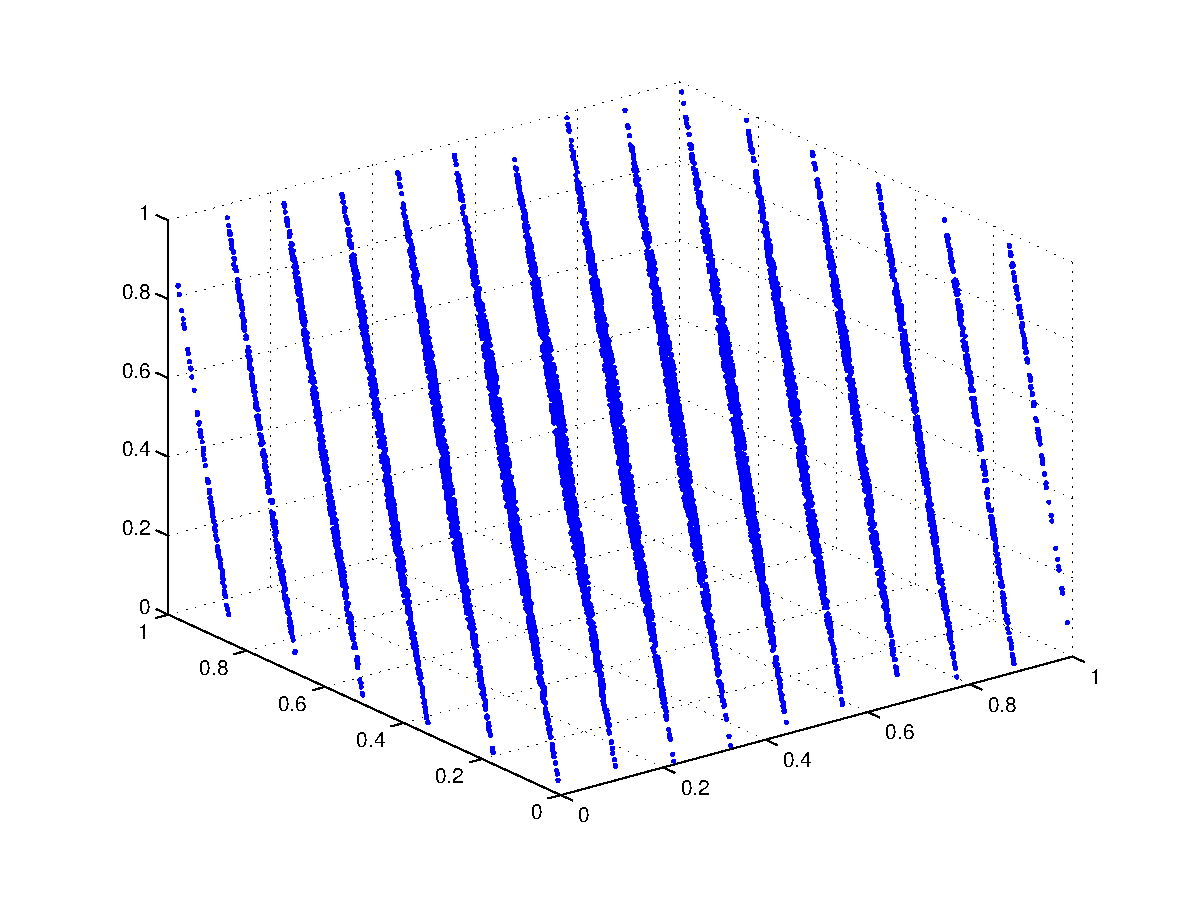
\includegraphics[width=8cm]{montecarlo/images/ibm_randu.eps}
	\caption{Verteilung aufeinanderfolgender Zufallszahlen des IBM Randu Algorithmus}
	\label{fig:IBMRandu}
\end{figure}

\subsubsection{Die rand() Funktion von C}
Durch die einfache und sehr effiziente Berechnung finden LCG
Generatoren viel Verbreitung in der Praxis. So verwendet die C-Funktion
\texttt{rand()} "ublicherweise den LCG-Algorithmus mit den Konstanten
$a=1103515245$, $c=12345$, $m=2^{31}$, und dem mit der Funktion
\texttt{srand()} gesetzten Startwert. \cite{rng:randFunction} Eine
g"angige Praxis ist es, den Startwert mit der aktuellen Systemzeit zu
initialisieren. Ein entsprechendes Code-Snippet liegt im Github-Repository
bei. \cite{rng:githubRepo}

Die \texttt{rand()} Funktion ist nicht genau spezifiziert ist und die
Periodendauer durch die Wahl von $m=2^{31}$ als Potenz von zwei eher
klein ist. Deshalb wird die Verwendung dieser Funktion nicht empfohlen.

\subsection{Lehmer Generator} \label{subsec:Lehmer}
Der Lehmer-Generator ist eine Unterart der LCG Generatoren, nach folgender
Rekursionsvorschrift:

\begin{equation}
	x_{i+1} = a x_{i} \mod{m}
	\label{equ:lehmer}
\end{equation}

wobei $m$ eine Primzahl sein muss. Sie zeichnen sich gegen"uber Standard
LCG Generatoren durch eine h"ohere Periodendauer aus. David W. Hutchinson
in seinem Paper \textit{``A new uniform pseudorandom number generator''}
1966 \cite{rng:Hutchinson1966} vor, das Modul  $m = 2^{31} - 1 =
2'147'483'647$ zu w"ahlen. Damit ist der Generator in 32-bit Systemen
relativ effizient umsetzbar. Eine optimale Wahl des Parameters $a$
blieb er jedoch schuldig. 

Erst Jahre sp"ater, im Oktober 1988, publizierten Stephen K. Park
und Keith W. Miller im Journal \textit{Communications of the
ACM}\footnote{Association for Computing Machinery: Renommierte
wissenschaftliche Gesellschaft zur F"orderung der Informatik} einen
Artikel \cite{rng:ParkMiller1988}, in welchem Sie genauer auf eine
gute Wahl von $a$ eingingen. Sie zeigten sich in ihrem Paper \textit{``
Random number generators: good ones are hard to find.''} sehr besorgt
"uber die g"angige Praxis von Zufallsgeneratoren - insbesondere auch in
Fach- und Lehrb"uchern:

\begin{quote}
\textit{Many generators have been written, most of them have demonstrably
non-random characteristics, and some are embarrassingly bad.}
\end{quote}
\begin{flushright}
	- Stephen Park, Keith Miller, 1988 \cite{rng:ParkMiller1988}
\end{flushright}

Sie kritisieren insbesondere, dass, wie am Beispiel IBM gezeigt, h"aufig
mehr Fokus auf Codeoptimierung anstatt auf die Qualit"at der Generatoren
gelegt wird. Neben der klaren Aussage, dass das Modul $m$ unbedingt eine
Primzahl sein soll, stellen Sie folgende Anforderungen an die Wahl des
Faktoren $a$:

\begin{enumerate}
\item Die Funktion $f(z) = a z \mod m$ erzeugt die maximal m"ogliche Periode $m$.
\item Die komplette erzeugte Sequenz ist zuf"allig.
\item $f(z)$ kann effizient auf einem 32-bit System implementiert werden.
\end{enumerate}

Aus Bedingung 3. folgt, dass die von Hutchinson \cite{rng:Hutchinson1966}
vorgeschlagene Wahl von $m = 2^{31} - 1$ fast optimal f"ur 32-bit Systeme
ist. Aus den mehr als 2 Milliarden m"oglichen $a$ erf"ullen nur einzelne
alle drei Bedingungen. Bereits 1969 schlugen Lewis, Goodman, Miller
\cite{rng:LewisGoodmanMiller1969} die Wahl von $a = 7^5 = 16'807$ vor,
bis zum Paper von Park und Miller fand dies aber kaum Beachtung. Genau
diese Kombination wurde von Park und Miller als \textbf{Minmal Standard}
f"ur Random Number Generators bezeichnet. In der Literatur wird f"ur
diesen RNG h"aufig die Bezeichnung Park-Miller RNG benutzt.

In den 90er Jahren wurde der Park-Miller Generator von einigen Seiten
kritisiert, sodass diese offiziell als neue Faktoren $a = 48271$ oder
$a = 69621$ empfahlen und ausdr"ucklich darauf hinwiesen dass der
Algorithmus nur als Minimal Standard zu verstehen ist. So hat sich
dieser auch weiterhin als Standard in vielen Bibliotheken etabliert
und ist eindeutig als schneller, einfacher, aber trotzdem qualitativ
hochwertiger RNG zu empfehlen.

\subsubsection{Implementation des Minimal Standard}
Eine logisch erscheinende Implementation in C sieht wie folgt aus:
\begin{lstlisting}[style=C]
	double random(int* seed) {
		const int a = 16807;
		const int m = 2147483647;
		
		*seed = (a * (*seed)) % m;
		return ((double)*seed) / m;
	}
\end{lstlisting}
wobei die Variable \texttt{seed} den aktuellen Integer Wert speichert,
und die Funktion \texttt{random} einen \texttt{double}-Wert zwischen
$0$ und $1$ zur"uckgibt. Auf den meisten Systemen wird diese Variante
\textbf{nicht} funktionieren. Der maximale Wert der Multiplikation
\texttt{a * (*seed)} betr"agt $16807*2147483646 \approx 1.03 * 2^{45}$,
was deutlich gr"osser als ein Integer ist. Um solche Fehler zu verhindern
schlagen Park und Miller vor, jede Implementation zu pr"ufen indem mit
$x_1 = 1$ der Wert $x_{10001} = 1043618065$ verifiziert wird.

Eine M"oglichkeit, solche Fehler zu umgehen liegt in der Verwendung
von Floating-Point Zahlen. Dabei ist anzumerken ist, dass der
Modulo-Operator f"ur Floating-Point in C nicht definiert ist,
sondern die Funktion \texttt{fmod()} aus dem \texttt{math.h} Header
verwendet werden muss. Trotzdem muss darauf geachtet werden, dass die
Mantisse mindestens 46-bit oder gr"osser ist, d.h. es muss bereits der
\texttt{double}-Datentyp\footnote{double: 52-bit Mantisse} anstelle von
\texttt{float}\footnote{float: 23-bit Mantisse} verwendet werden.

Der deutlich elegantere Ansatz ist es, jegliche Werte kleiner als $2^{32}$
zu halten. Dazu wird $m$ geschrieben als

\begin{equation}
	m = aq + r
\end{equation}
mit 
\begin{equation}
	q = \lfloor m/a \rfloor \qquad \text{und} \qquad r = m \text{ mod } a
\end{equation}
Daraus ergibt sich: (Beweis, siehe \cite{rng:ParkMiller1988})
\begin{equation}
	a x \text{ mod } m = 
		\begin{cases}
			a \left(x \text{ mod } q\right) - r \lfloor x / q\rfloor & \text{wenn }\geq 0 \\
			a \left(x \text{ mod } q\right) - r \lfloor x / q\rfloor + m & \text{sonst}
		\end{cases}
\end{equation}
Damit ergeben sich Zwischenresultate bis $2^{32}$, womit eine einfache
Implementation m"oglich ist:

\begin{lstlisting}[style=C]
	double random(int* seed) {
		const int a = 16807;
		const int m = 2147483647;
		const int q = 127773;
		const int r = 2836;
		
		int k = *seed / q;
		*seed = a * (*seed - k*q) - k*r;
		if(*seed < 0)   *seed += m;
		return (double)*seed / m;
	}
\end{lstlisting}
Diese Implementation ist nicht nur sehr schnell, sondern verf"ugt, wie
von Park und Miller \cite{rng:ParkMiller1988} nachgewiesen, "uber sehr
gute Eigenschaften um als Minimal Standard verwendet zu werden.

\subsection{Mersenne-Twister} \label{subsec:MersenneTwister}
Der Mersenne-Twister Algorithmus zeichnet sich durch eine extrem
hohe Periode von $2^{19937}-1 \approx 4.3 \cdot 10^{6001}$ aus. Die
Periodenl"ange ist eine Mersenne-Primzahl\footnote{Mersenne-Primzahl:
Primzahl der Form $2^{n}-1$} und gibt dem Algorithmus den Namen. Die
Ausgabesequenz ist bis zur Dimension 623 gleichverteilt, d.h. werden
die ausgegebenen Zahlen als Vektoren bis Dimension 623 interpretiert,
so sind diese Vektoren immer gleichverteilt.

Der Mersenne-Twister Algorithmus arbeitet mit 624 Zustandsw"ortern
$Y_1 \dots Y_N$ von typischerweise 32-bit L"ange. Diese Zust"ande
werden zu Beginn des Algorithmus initialisiert. Dies wird h"aufig mit
dem in Abschnitt \ref{subsec:RandomDev} beschriebenen Random-Device
oder mit einfacheren Zufallszahlgeneratoren wie dem LCG gemacht. Je
besser (d.h. zuf"alliger) die Initialisierung, desto fr"uher sind die
generierten Zahlen auch zuf"allig. Ist dies nicht gew"ahrleistet, kann
$Y[2]$ mit einem zuf"alligen Seed, z.B. der Uhrzeit, initialisiert
werden und $800\text{\strut'}000$ Zahlen generiert werden, bevor der Algorithmus
benutzt wird. So ist eine gute Gleichverteilung sichergestellt.

Der Algorithmus f"ur alle darauf folgenden Zufallszahlen $Y_i$ f"ur
$i>N$ werden wie folgt berechnet\footnote{$\oplus$: XOR-Funktion,
$\wedge$: And-Funktion}:

\begin{align}
	h &:=  Y_{i-N} - Y_{i-N} \mod{2^{31}} + Y_{i-N+1} \mod{2^{31}} \\
	Y_i &:= Y_{i-227} \oplus \left\lfloor \frac{h}{2} \right\rfloor \oplus \left( \left(h \mod{2} \right) \cdot 9908b0df_{\text{hex}}\right)
\end{align}

Um sicherzustellen, dass alle 32-bit gleichverteilt sind, werden die
Zufallszahlen $Z$ aus $Y$ wie folgt berechnet:
\begin{align}
	x &:= Y_{i} \oplus \left\lfloor \frac{Y_i}{2^{11}} \right\rfloor \\
	y &:= x \oplus \left(\left(x \cdot 2^7\right) \wedge 9d2c5680_{\text{hex}} \right) \\
	z &:= y \oplus \left(\left(y \cdot 2^{15}\right) \wedge efc60000_{\text{hex}} \right) \\
	Z_i &:= z \oplus \left\lfloor \frac{z}{2^{18}} \right\rfloor
\end{align}

Obwohl der Mersenne-Twister Algorithmus sehr kompliziert scheint,
ist die Ausf"uhrung sehr schnell, weil fast nur Additionen und
Bit-weise Manipulationen ausgef"uhrt werden. Zusammen mit den bereits
beschriebenen Vorteilen hat dies dazu gef"uhrt, dass der Mersenne-Twister
der Standard-Zufallszahlengenerator in vielen Bibliotheken, wie z.B. der
\textit{GNU Scientific Library} ist.


\subsection{Erzeugen bestimmter Verteilungen}
Wie unter \ref{subsec:numIntegration} ausgef"uhrt, werden Integrale
h"aufig mit der Monte Carlo Methode gel"ost, indem Zufallszahlen mit einer
bestimmten Verteilung generiert werden. Es werden also Methoden ben"otigt,
beliebige Verteilungen zu erreichen. Obwohl verschiedene M"oglichkeiten
bestehen, ist es nat"urlich nicht m"oglich, alle Verteilungen mit
vern"unftigem Aufwand zu erreichen. Die einfachste Methode ist die im
folgenden Abschnitt beschriebene Inversionsmethode.

\subsubsection{Inversionsmethode}

Um aus der im Einheitsintervall $[0,1]$ gleichverteilten Zufallsvariable
$z$  eine Zufallsvariable $x$ mit der Verteilungsfunktion $F_X(x)$
zu erhalten, muss F invertiert werden und auf $z$ angewandt werden.

\begin{equation}
	x = F^{-1}(z)
\end{equation}

Ist die Inversion von $F$ analytisch m"oglich, ist diese Methode einfach
anwendbar. Es ist zwar m"oglich, $F$ numerisch zu invertieren, was jedoch
h"aufig aufw"andiger ist als die Anwendung anderer Methoden.

In Tabelle \ref{tab:verteilungen_erzeugen} sind die mit der
Inversionsmethode erstellten Algorithmen zum Generieren von Zufallszahlen
einiger ausgew"ahlter Verteilungen aufgestellt.

\begin{table}[htbp]
	\centering
	\renewcommand{\arraystretch}{1.5}
	\begin{tabular}{|l|l|l|}
		\hline
		Wahrscheinlichkeitsdichte & Wertebereich & Algorithmus \\ \hline
		$f(x) = \frac{1}{b-a}$ & $[a,b[$ & $x = (b-a) \cdot z + a$ \\ \hline
		$f(x) = 2x$ & $[0,1]$ & $x = \sqrt{z}$ \\ \hline
		$f(x) = \frac{1}{k} \exp^{-x/k}$ & $]0,\infty]$ & $x = -k \ln z$ \\ \hline
		$f(x) = - \ln x$ & $[0,1[$ & $x = z_1 \cdot z_2$ \\ \hline
	\end{tabular}
	\caption{Algorithmen zur Erzeugung von Zufallszahlen $x$ aus in $[0,1]$ gleichverteilten Zufallsvariablen $z$.}
	\label{tab:verteilungen_erzeugen}
	\renewcommand{\arraystretch}{1.0}
\end{table}

\subsection{Implementation mit Boost}
Die C++ Bibliothek \textit{Boost} bietet sehr gute M"oglichkeiten zum
Generieren von Zufallszahlen. Es lassen sich oben vorgestellte, wie auch
verschiedene weitere Generatoren ausw"ahlen. Auch die Verteilungsfunktion
kann frei gew"ahlt werden.

Um einen Zufallszahlengenerator zu erstellen wird als erstes eine
Klasse vom gew"unschten Generatortypen instanziert. Hier wird z.B. ein
Mersenne-Twister mit der aktuellen Systemzeit als Seed erstellt.

\begin{lstlisting}[style=C]
static mt19937 gen(time(0));
\end{lstlisting}

Darauf wird ausgew"ahlt, welche Verteilungsfunktion verwendet wird. Hier
wird eine Gleichverteilung im Intervall $[0,1[$ erzeugt.

\begin{lstlisting}[style=C]
static uniform_01<mt19937> dist(gen); 
\end{lstlisting}

Darauf kann die Funktion \texttt{dist()} verwendet werden um
Zufallszahlen zu generieren. Der komplette Code ist im Github-Repository
\cite{rng:githubRepo} abgelegt.

Detaillierte Informationen zu den M"oglichkeiten mit der Boost
Random-Funktion ist auf der entsprechenden Referenz-Seite zu finden
\cite{rng:boostRandom}.



\newpage
\printbibliography[heading=subbibliography]
\end{refsection}
